\section{Simulation Analysis}
\label{sec:simulation}

\subsection{Transient analysis}

We simulated the circuit using transient analysis, using a non ideal transformer and the following components:

\begin{table}[H]
\addtolength{\tabcolsep}{-4pt}
\caption{Valores de $I$ e $V$ para cada ensaio}
\vspace{-3mm}
\begin{tabular}{|c|c|c|}
\hline
C1 & $3.7224\miu F$ \\
R1 & $3.7224k\Ohm$ \\
C2 & $15\miu F$ \\
R2 & $15k\Ohm$ \\
C3 & $10\miu F$ \\
R3 & $10k\Ohm$ \\
\hline
\end{tabular}
\label{tab:Components}
\end{table}

\par

Firstly we simulate the initialization of the circuit, and only once it has stabelized do we take the average and ripple of $V_{out}$. Ploting the potential of the rectifier circuit, the envelope detector circuit and $V_{out}$ for the first 2 seconds.

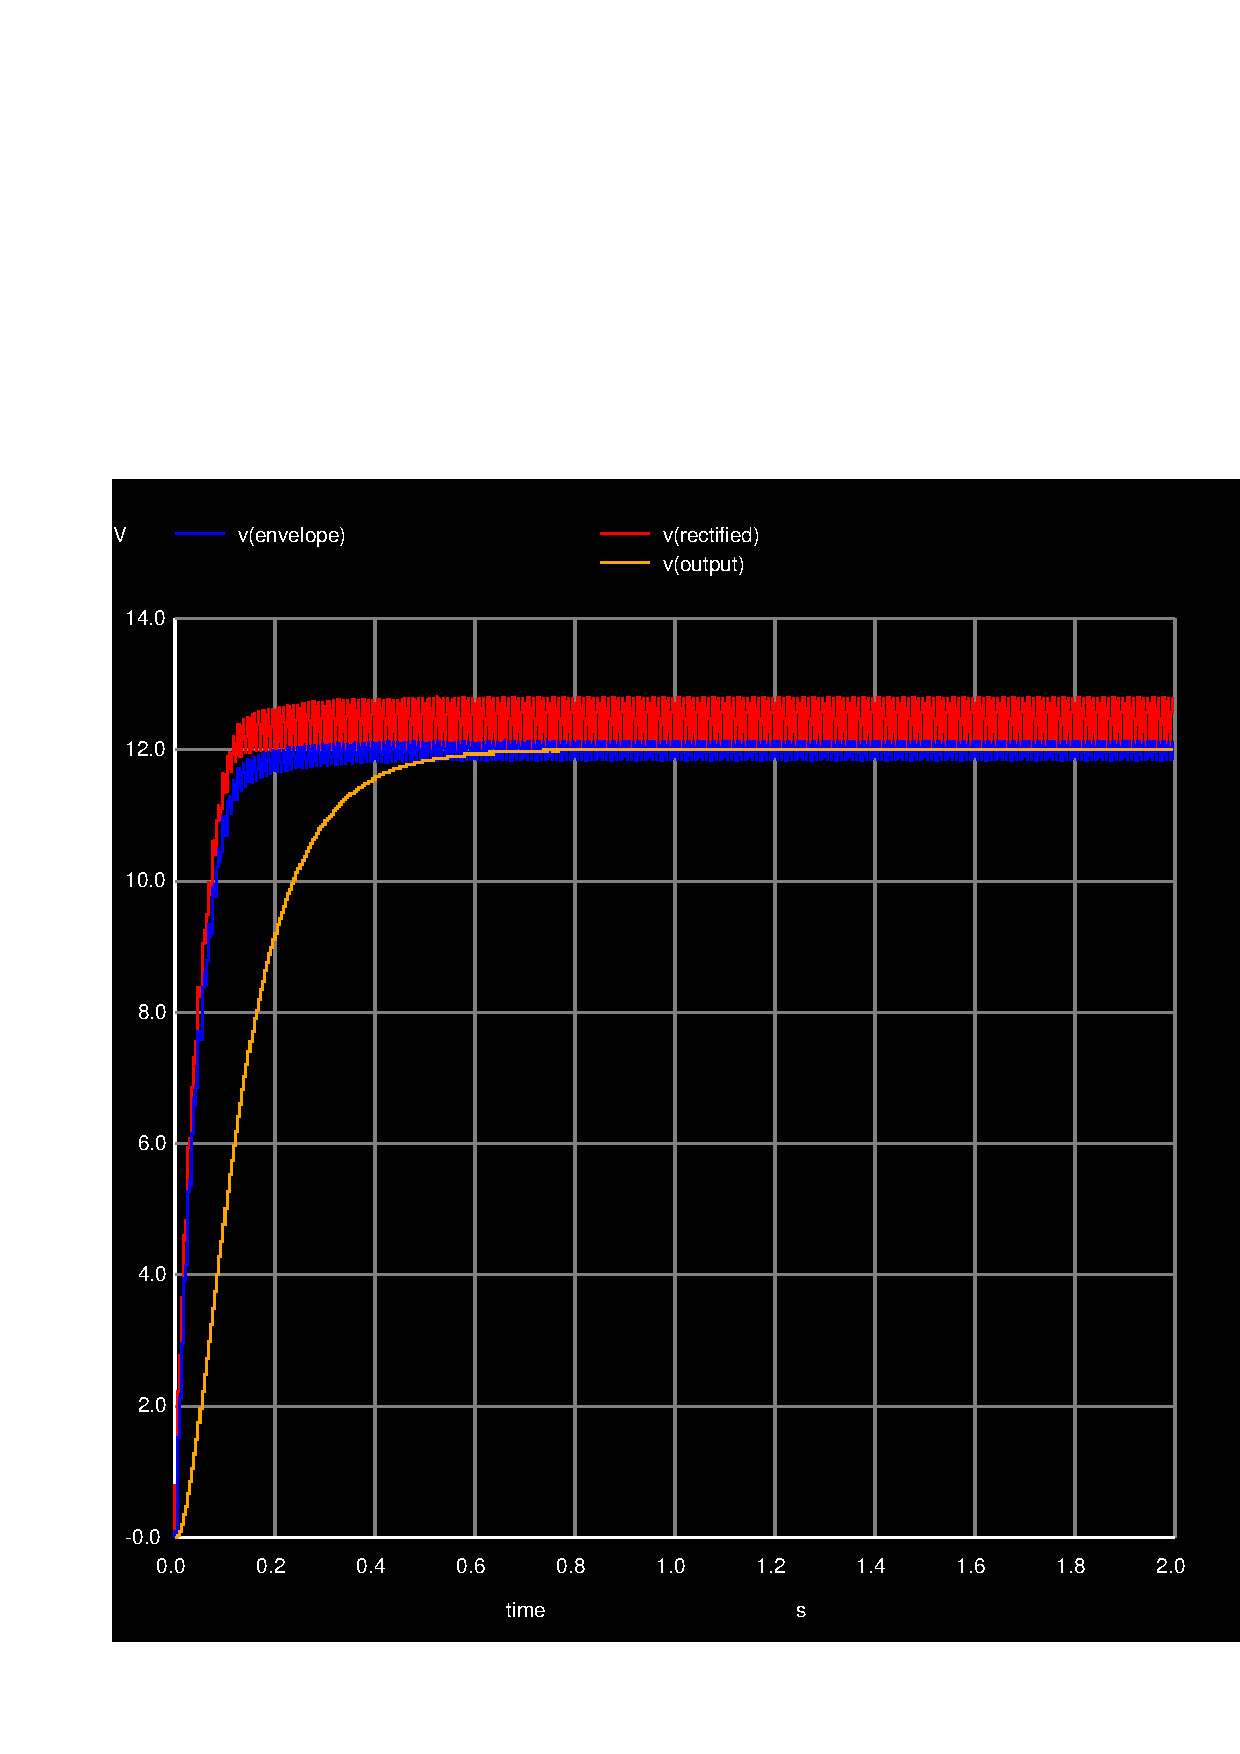
\includegraphics[width=1\linewidth]{../sim/vinit.pdf}

As we can observe, the stabilization time for $V_{out}$ is approximatly 0.6 seconds, but the start-up sequence always has a lower voltage than the desired output, so it doesn't pose a threat to damage the circuit connected to the output.

\par

By choosing a 10 period section in which the circuit has already stabelized, we can better study it.

\begin{minipage}[c]{0.50\linewidth}
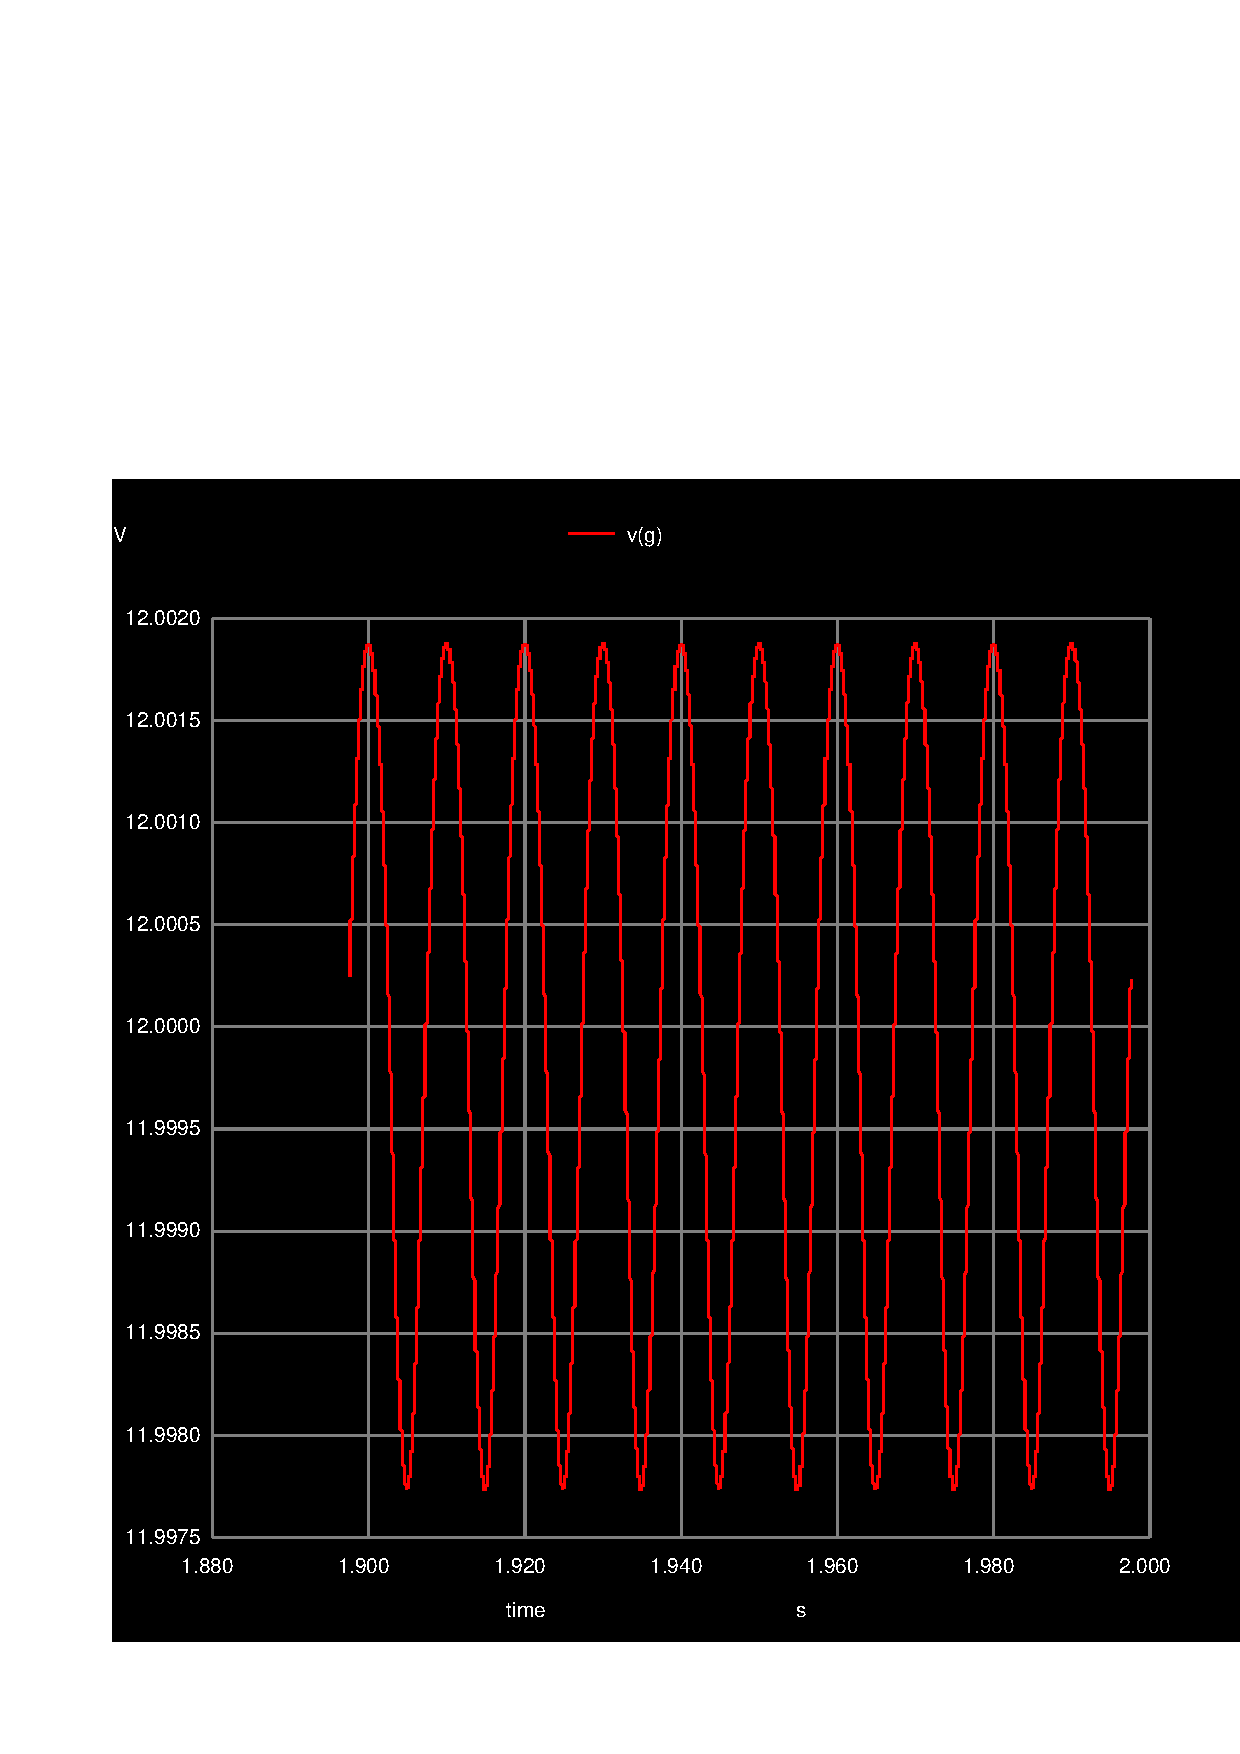
\includegraphics[width=1\linewidth]{../sim/vout.pdf}
\end{minipage} % no space if you would like to put them side by side
\hspace{1mm}
\begin{minipage}[c]{0.50\linewidth}
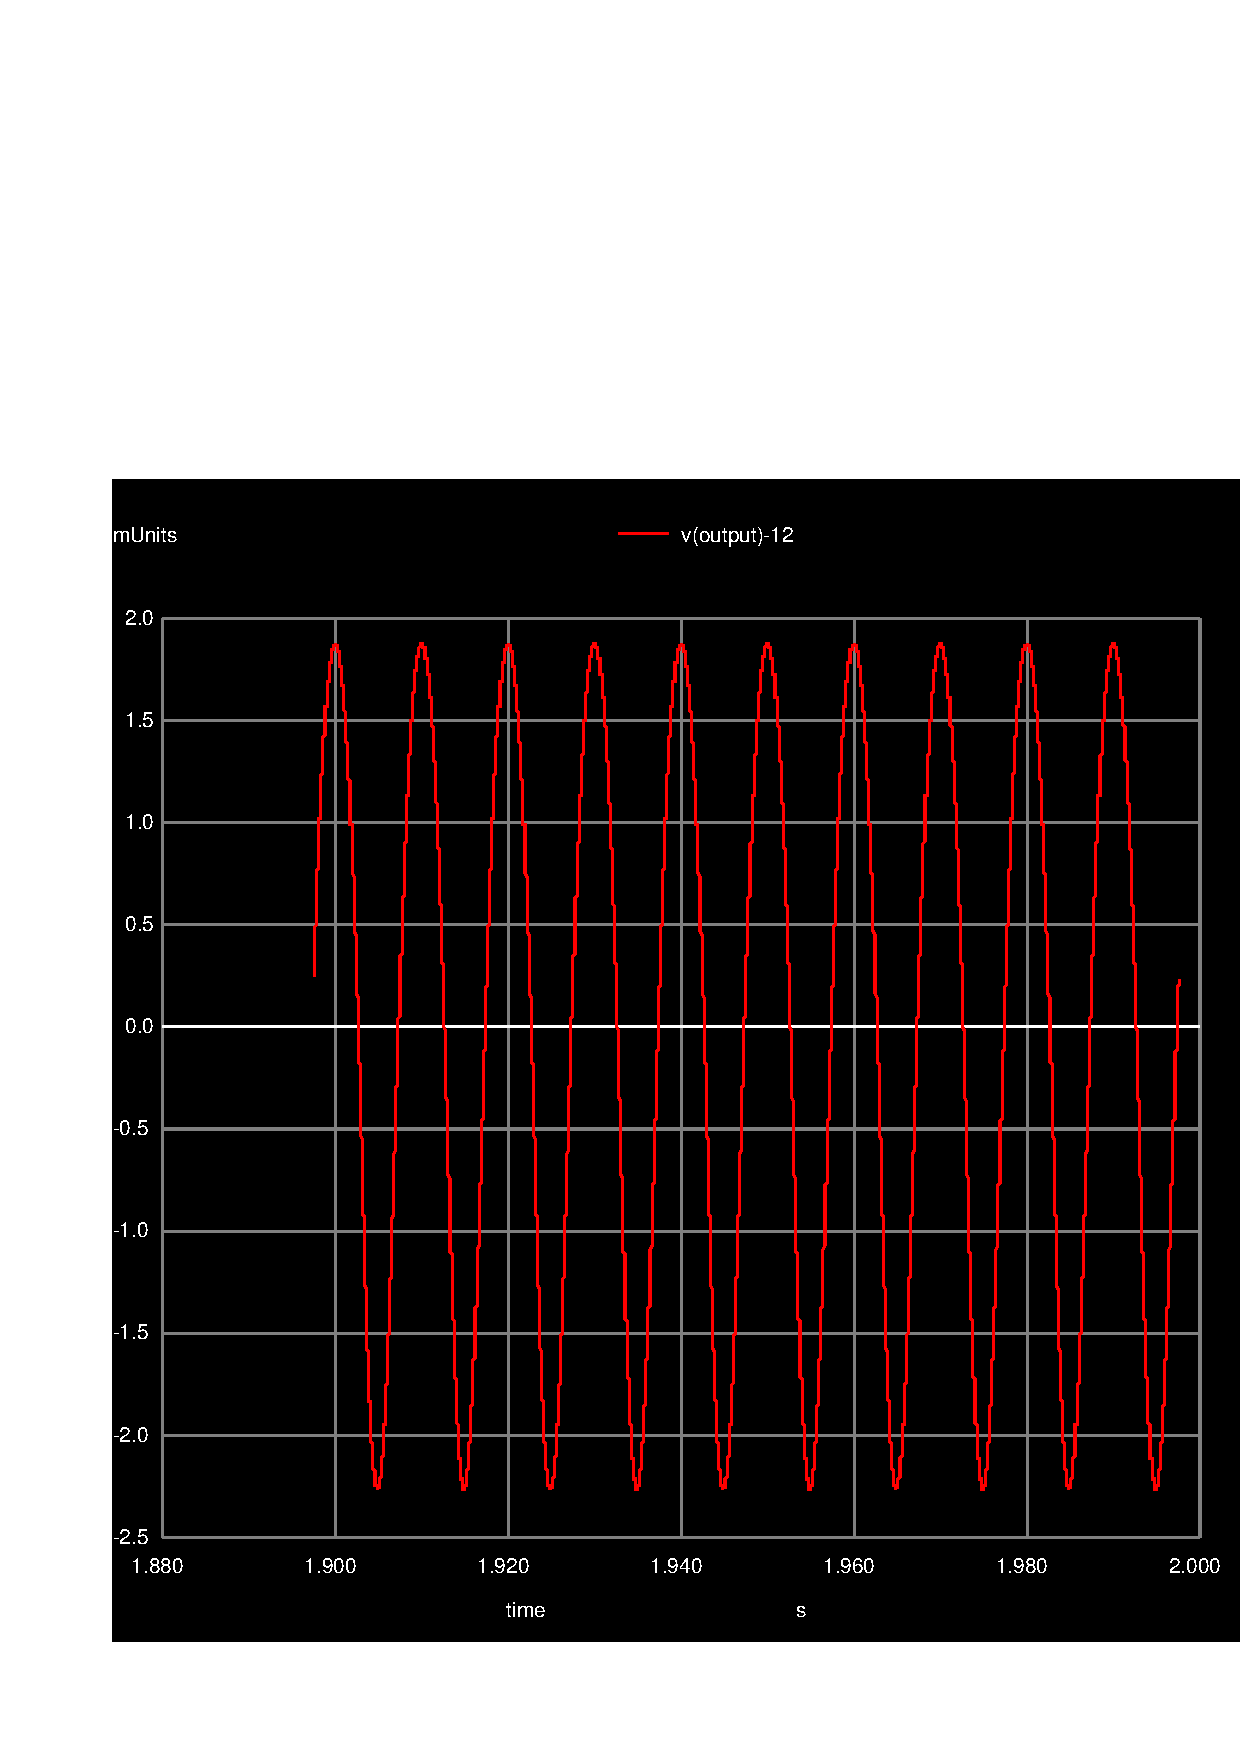
\includegraphics[width=1\linewidth]{../sim/v12.pdf}
\end{minipage}
    
The average of $V_{out}$ in equilibrium is 12.000000V and the ripple is 4.13 mV. The circuit costs 59.9448 monetary units, and the calculated merit is 4.038251.
